\documentclass[pmlr]{jmlr}

% ---------------------------------------------------------------
% MLHC 2026 requires 11-point Times font.
% newtxtext/newtxmath provide Times Roman text + matching math.
% ---------------------------------------------------------------
\usepackage{txfonts}  % Times Roman text and math fonts (11pt per MLHC requirement)

% ---------------------------------------------------------------
% Packages (jmlr auto-loads: amsmath, amssymb, natbib, graphicx,
%           url, algorithm2e — add only extras here)
% ---------------------------------------------------------------
\usepackage{booktabs}
\usepackage{longtable}
\usepackage{capt-of}
\usepackage{mathtools}
\usepackage{multirow}
\usepackage{array}
\usepackage{enumitem}
\usepackage{float}
\usepackage{placeins}
\usepackage{tikz}
\usetikzlibrary{arrows.meta,positioning,fit,calc,shapes.multipart}
% hyperref is loaded by jmlr.cls -- removed to avoid option clash

% siunitx workaround for newer LaTeX releases
\makeatletter
\def\set@curr@file#1{\def\@curr@file{#1}}
\makeatother
\usepackage[load-configurations=version-1]{siunitx}

% ---------------------------------------------------------------
% MLHC-specific metadata
% ---------------------------------------------------------------
\jmlrvolume{[VOLUME \# TBD]}
\jmlryear{2026}
\jmlrworkshop{Machine Learning for Healthcare}

% ---------------------------------------------------------------
% Title  (ANONYMIZED for double-blind review)
% ---------------------------------------------------------------
\title{%
 Amortized Data Borrowing with Exchangeability-Aware Neural Posterior Estimation}

% Author block MUST be left blank for anonymous submission.
% Replace with real names/affiliations only in the camera-ready version.
\author{%
  \Name{Anonymous Author(s)}
  \Email{anonymous@anonymous.edu}\\
  \addr Anonymous Institution
}

% ---------------------------------------------------------------
\begin{document}
\maketitle

\begin{abstract}
Leveraging external or historical cohorts to augment small concurrent studies
is attractive in Alzheimer's disease research, where longitudinal follow-up is
expensive and disease trajectories are heterogeneous.
Bayesian dynamic borrowing (BDB) provides a principled mechanism for
adaptively controlling the influence of external data, but classical
implementations often rely on hand-tuned low-dimensional summaries and can be
computationally expensive when posterior computation is repeated for each new
dataset pair.
We study amortized neural posterior estimation (NPE) as a flexible alternative
for dynamic borrowing under cohort shift.
The method is pretrained on simulated current/external dataset pairs and
then produces an approximate posterior for the current-study estimand with a
single forward pass.
We evaluate the approach in a controlled simulation study spanning six
exchangeability regimes, including covariate shift, outcome drift, and joint
non-exchangeability, and compare against representative dynamic borrowing and
reweighting baselines.
NPE is not uniformly best in easy exchangeable settings, but it is more stable
when outcome drift or joint covariate/outcome mismatch causes classical
borrowing rules to become biased and anti-conservative.
After pretraining, NPE also returns posterior summaries in milliseconds, while
MCMC-based borrowing baselines require repeated posterior sampling to certify
joint posterior quality.
We then present a real-world case study using the Alzheimer's Disease
Neuroimaging Initiative (ADNI), treating ADNI1 as an external cohort and
ADNIGO/ADNI2 as the concurrent cohort among baseline mild cognitive impairment
subjects.
The ADNI application is not a randomized treatment-effect analysis; instead,
it is a real-data borrowing example in which event-rate differences make naive
borrowing poorly calibrated.
Together, the simulation and ADNI results suggest that amortized posterior
estimation is most useful when source mismatch is difficult to capture with a
fixed borrowing rule, while retaining fast reusable inference after
pretraining.
\end{abstract}

\section{Introduction}
to fix
External or historical cohorts are increasingly used to augment small
concurrent studies in medicine.
When the external and concurrent sources are sufficiently similar, borrowing
can improve efficiency and stabilize estimation.
When the sources differ in meaningful ways, however, naive borrowing can
introduce bias and distort uncertainty quantification
\citep{viele2014use}.
This tension is especially important in Alzheimer's disease research, where
prospective follow-up is expensive, clinically meaningful outcomes accrue
slowly, and related cohorts often differ in enrollment criteria, disease
severity, and assessment practice.

Bayesian dynamic borrowing (BDB) provides a principled framework for
adaptively controlling how much external information should influence
current-study inference
\citep{ibrahim2000power,hobbs2011commensurate,neuenschwander2010summarizing,
schmidli2014robust}.
Classical BDB methods such as the power prior, commensurate prior, and robust
MAP prior have strong statistical motivation, but in practice they still
require repeated model fitting for each new dataset pair and often summarize
cross-source compatibility through one or a few low-dimensional quantities.
That can be restrictive in settings where source mismatch is multi-faceted.

Amortized neural posterior estimation (NPE) offers a different route.
Instead of rerunning MCMC or numerical optimization for every new
current/external pair, the idea is to train a neural network offline on many
simulated borrowing problems and then use the trained network to output an
approximate posterior in a single forward pass
\citep{papamakarios2019sequential,greenberg2019automatic,cranmer2020frontier,
lueckmann2021benchmarking}.
The key design question is how to represent the two sources so that the
network sees both the target estimand and the degree of non-exchangeability.

In this paper we focus on a summary-based NPE approach for dynamic borrowing.
We first study the method in a controlled simulation setting spanning six
exchangeability regimes, including covariate shift, outcome drift, and joint
non-exchangeability.
We then examine a real-data borrowing case study using the Alzheimer's Disease
Neuroimaging Initiative (ADNI) \citep{petersen2010alzheimer,weiner2017alzheimer}.
Specifically, ADNI1 is treated as an external cohort and ADNIGO/ADNI2 as a
concurrent cohort among baseline mild cognitive impairment (MCI) subjects, with
24-month conversion to dementia as the outcome.
This real-world application is not presented as a randomized treatment-effect
analysis; rather, it is used to study borrowing under cohort shift in a
clinically meaningful longitudinal dataset.

The ADNI application serves two purposes.
First, it provides an empirical check that the borrowing problem is real in
practice: the external and concurrent cohorts have different event rates and
therefore are not directly exchangeable.
Second, it gives a setting in which we can adapt the NPE framework to infer a
concurrent risk-level parameter while allowing the external cohort to differ
through a nuisance shift parameter.
This keeps the spirit of dynamic borrowing while avoiding an overstatement
that the real-data example exactly matches the treatment-effect simulations.

The remainder of the paper is organized as follows.
Section~\ref{sec:related} reviews dynamic borrowing, balancing methods, and
simulation-based inference.
Section~\ref{sec:problem} introduces the simulation regimes and the ADNI
borrowing setup.
Section~\ref{sec:figures_plan} presents the empirical design, summarizes the
current simulation workflow, and reports the ADNI real-world application.

% -------------------------------------------------------
% REQUIRED MLHC SECTION
% -------------------------------------------------------
\subsection*{Generalizable Insights about Machine Learning in the Context
             of Healthcare}

\begin{itemize}[leftmargin=1.5em, itemsep=2pt]
  \item \textbf{Amortized inference can make adaptive borrowing practical in
        healthcare studies with repeated external comparisons.}
        Training an NPE model offline allows approximate posterior inference
        for new cohort pairs without rerunning expensive Bayesian computation
        from scratch each time.

  \item \textbf{Real-world borrowing problems often appear first as calibration
        mismatch rather than discrimination failure.}
        In the ADNI application, external-only models rank subjects well but
        systematically overestimate risk in the concurrent cohort, showing that
        borrowing decisions should account for cohort shift even when predictive
        AUC remains high.

  \item \textbf{A combined simulation-plus-case-study design is useful for
        evaluating healthcare borrowing methods.}
        Controlled simulations make it possible to assess bias and error under
        known exchangeability violations, while a real-world case study checks
        whether the same issues appear in practice and whether the method
        behaves sensibly on clinically meaningful data.
\end{itemize}

\section{Related Work}
\label{sec:related}

\subsection{Bayesian dynamic borrowing and the exchangeability assumption}

Integrating external information into a concurrent study has a long history
in clinical biostatistics, beginning with the hierarchical framework of
\citet{pocock1976combination} for combining randomized and historical
controls.
Let $D_c$ denote the data from a small current study and $D_e$ the data from
an external or historical source, with a current-study target parameter
$\theta$.
The central statistical assumption underlying any borrowing procedure is
\emph{exchangeability} between the two sources: that, conditional on
covariates, observations from $D_c$ and $D_e$ share a common generative
mechanism.
When exchangeability holds, pooling reduces variance and improves
precision, yielding effective sample-size gains that are especially valuable
in rare-disease, pediatric, and oncology trials where concurrent accrual is
limited \citep{berry2013bayesian,ventz2019design,edwards2024using}.
When it fails---because of secular drift, differing diagnostic criteria, or
changes in the outcome mechanism---naive pooling induces bias and can inflate
type~I error \citep{viele2014use,koppschneider2020power,psioda2019bayesian}.
This tension motivates \emph{dynamic} rather than fixed borrowing: methods
that quantify cross-source compatibility and modulate the contribution of
$D_e$ accordingly.
Existing dynamic borrowing methods mainly differ in how they assess
compatibility between $D_c$ and $D_e$ and how that assessment is translated
into borrowing strength.

\paragraph{Power prior.}
The power prior \citep{ibrahim2000power,ibrahim2015power} incorporates
external information by discounting the external likelihood through a scalar
weight $a_0 \in [0,1]$:
\begin{equation}
p(\theta \mid D_c, D_e, a_0)
\;\propto\;
L(\theta; D_c)\,L(\theta; D_e)^{a_0}\,\pi(\theta).
\end{equation}
When $a_0 = 1$ the two sources are fully pooled, whereas $a_0 = 0$ ignores
the external data entirely.
Fixing $a_0$ a priori is difficult in practice.
The normalized power prior \citep{duan2006evaluating,ye2022normalized} treats
$a_0$ as unknown and integrates over it, and empirical-Bayes adaptive
variants \citep{gravestock2017adaptive} plug in a data-driven estimate.

\paragraph{Commensurate prior.}
The commensurate prior \citep{hobbs2011commensurate,hobbs2012commensurate}
introduces separate parameters for the current and external sources and
links them through a precision parameter $\tau$:
\begin{align}
\theta_e &\sim \pi(\theta_e), &
\theta_c \mid \theta_e, \tau &\sim \mathcal{N}(\theta_e,\tau^{-1}).
\end{align}
Large $\tau$ encourages $\theta_c$ and $\theta_e$ to be close, whereas small
$\tau$ allows them to differ.
With an appropriate hyperprior on $\tau$, the posterior adaptively reduces
borrowing under prior--data conflict \citep{evans2006checking,
presanis2013conflict}.

\paragraph{Meta-analytic-predictive and robust MAP priors.}
The meta-analytic-predictive (MAP) prior
\citep{neuenschwander2010summarizing} derives an informative prior for
$\theta_c$ by treating historical trials as exchangeable draws from a common
hierarchical model.
Because exchangeability can fail in ways that are hard to anticipate,
\citet{schmidli2014robust} proposed a robust MAP prior that mixes the
informative component with a vague one:
\begin{equation}
\pi_{\text{robust}}(\theta_c)
=
(1-\epsilon)\,\pi_{\text{MAP}}(\theta_c)
+
\epsilon\,\pi_{\text{vague}}(\theta_c),
\end{equation}
where $\epsilon$ controls protection against conflict between historical and
current data.
This construction is attractive in practice because $\epsilon$ has a
transparent interpretation, but the choice of $\epsilon$ and of the vague
component materially affects the resulting borrowing behavior.

\paragraph{Limitations of classical BDB.}
Several studies have documented recurring practical limitations of these
methods.
First, operating characteristics are sensitive to the discount
hyperparameters $(a_0,\tau,\epsilon)$, and strict type~I error control
essentially eliminates the power gains that motivated borrowing in the first
place \citep{koppschneider2020power,galwey2017supplementation,
vanrosmalen2018including}.
Second, classical BDB methods summarize cross-source compatibility through
\emph{one or a few low-dimensional quantities}, which can mask clinically
important source differences: in particular, covariate shift and outcome
drift enter the same scalar $a_0$ or $\tau$, even though they have very
different implications for bias in the current-study estimand
\citep{viele2014use,dahabreh2019generalizing}.
Third, these models require repeated posterior fitting---typically via
MCMC---for each new dataset pair, which is expensive when operating
characteristics must be simulated across many scenarios, when borrowing
decisions must be reassessed for several candidate external cohorts, or when
the analysis must be rerun as data accrue.
These limitations motivate borrowing procedures that can (i) exploit richer,
multi-dimensional summaries of source compatibility, and (ii) amortize
inference cost across many current/external pairs.

\subsection{Balancing and reweighting methods}

A related class of methods approaches external-data use through balancing or
reweighting rather than hierarchical priors.
Propensity-score matching and weighting
\citep{rosenbaum1983central,stuart2010matching} adjust the external cohort so
that its covariate distribution better matches the current cohort.
Inverse-probability weighting is a standard implementation but can be
unstable when estimated propensity scores are close to 0 or 1
\citep{chesnaye2022introduction}, and overlap weighting
\citep{li2018balancing,li2019addressing} addresses this instability by
emphasizing subjects in the region of covariate overlap, with weights
proportional to $2\hat e(x)(1-\hat e(x))$.
Entropy balancing \citep{hainmueller2012entropy} reweights the external
cohort to match prespecified moments of the current cohort without estimating
a propensity model.
These ideas extend naturally to transportability and generalizability of
causal estimands across populations
\citep{dahabreh2019generalizing}.
Regulators have also begun to formalize the use of external and synthetic
controls in pivotal studies \citep{thorlund2020synthetic,fda2023external}.

A key limitation of weighting-based approaches, however, is that they
primarily address differences in baseline \emph{covariates} but not
differences in the \emph{outcome} generation mechanism
\citep{viele2014use,dahabreh2019generalizing}.
In Alzheimer's cohorts in particular, an external and a current source can
also differ in recruitment period, diagnostic practice, assessment schedule,
and baseline conversion risk.
In that case, balancing baseline covariates may not be enough: even a
well-calibrated external model may encode a shifted outcome relationship
relative to the current cohort.
This calibration-level mismatch, rather than covariate imbalance, is the
dominant failure mode in our ADNI case study.

\subsection{Neural posterior estimation and simulation-based inference}

Simulation-based inference (SBI) is a family of methods that perform
Bayesian inference using only the ability to simulate from the generative
model \citep{cranmer2020frontier}.
Neural posterior estimation (NPE) is the branch of SBI that trains a
conditional density estimator $q_{\phi}(\theta \mid x)$ directly on
simulated parameter--data pairs
\citep{papamakarios2016fast,papamakarios2019sequential,greenberg2019automatic,
lueckmann2021benchmarking}, with training objective
\begin{equation}
\mathcal{L}(\phi)
=
\mathbb{E}_{\theta \sim \pi(\theta),\, x \sim p(x\mid \theta)}
\left[-\log q_{\phi}(\theta \mid x)\right].
\end{equation}
Once trained, the network can produce an approximate posterior for a new
observation in a single forward pass, avoiding repeated posterior sampling.
Normalizing flows are the standard choice for $q_\phi$ because they provide
flexible, exactly-evaluable densities
\citep{papamakarios2021normalizing}, and open-source toolkits such as
\texttt{sbi} \citep{tejerocantero2020sbi} and \texttt{BayesFlow}
\citep{radev2022bayesflow} have made these methods practical for scientific
applications ranging from neuroscience \citep{goncalves2020training} to
epidemiology.

Two features of NPE are directly relevant to dynamic borrowing.
First, inference is \emph{amortized}: the upfront simulation-and-training
cost can be reused across many new dataset pairs, which matches the setting
where the same borrowing procedure must be evaluated repeatedly as cohorts
change.
Second, the network's input can be any summary of the two sources, not just
a single compatibility scalar---so long as the simulator covers the
relevant exchangeability regimes.
This expands the representational budget that governs how borrowing strength
reacts to different kinds of cohort shift.

For dynamic borrowing, the representation supplied to the posterior
estimator must therefore encode both information about the target estimand
and information about \emph{source compatibility}.
This requirement differs from many standard SBI settings, in which the
primary challenge is compressing data without losing information about a
single target parameter.
In borrowing problems, the representation must additionally preserve
structure that is informative about when external data should and should
not influence inference---the perspective we take in the remainder of the
paper.

\section{Background and Problem Setup}
\label{sec:problem}

\subsection{Dynamic borrowing setup}

Let
\[
D_c = \{(x_{ci}, y_{ci})\}_{i=1}^{n_c}
\quad \text{and} \quad
D_e = \{(x_{ej}, y_{ej})\}_{j=1}^{n_e}
\]
denote the concurrent and external datasets, respectively.
The inferential goal is always defined with respect to the concurrent
population.
External data can be useful when it is sufficiently compatible with the
concurrent cohort, but should be downweighted or ignored when the two sources
are not exchangeable.

In the stylized simulation study, the target estimand is a scalar
current-study treatment effect $\theta$.
The NPE method receives fixed-length summary statistics computed from
$(D_c, D_e)$ and returns an approximate posterior
\[
q_{\phi}(\theta \mid s(D_c, D_e))
\approx
p(\theta \mid D_c, D_e),
\]
where $s(D_c, D_e)$ contains source-level summaries and mismatch diagnostics.
This preserves the core dynamic borrowing goal while replacing repeated
per-dataset Bayesian fitting with amortized posterior inference.

\subsection{Exchangeability regimes}

The simulation study is organized around six regimes designed to stress-test
borrowing methods under distinct forms of source mismatch:

\begin{center}
\begin{tabular}{>{\raggedright\arraybackslash}p{0.14\linewidth}
                p{0.78\linewidth}}
\toprule
Scenario & Interpretation \\
\midrule
SC1 & \textbf{All exchangeable.}
      The external and concurrent cohorts have similar covariate distributions
      and the same outcome mechanism. \\[2pt]
SC2 & \textbf{Partial covariate shift.}
      Moderate differences in covariate distributions with a similar outcome
      mechanism. \\[2pt]
SC3 & \textbf{Partial outcome drift.}
      Covariate distributions are similar, but the outcome mechanism differs
      moderately. \\[2pt]
SC4 & \textbf{Strong covariate shift.}
      The external cohort differs substantially in case mix. \\[2pt]
SC5 & \textbf{Strong outcome drift.}
      Covariate distributions are similar, but the outcome mechanism differs
      materially. \\[2pt]
SC6 & \textbf{Joint non-exchangeability.}
      Both the covariate distribution and the outcome mechanism differ. \\
\bottomrule
\end{tabular}
\end{center}

These regimes deliberately separate settings in which mismatch is mainly
covariate-driven from settings in which it is mainly outcome-driven.
They provide a common evaluation grid for both classical borrowing methods and
the amortized NPE estimator.

\subsection{Summary-based neural posterior estimation}

The NPE model operates on a fixed-length summary vector
\[
s(D_c, D_e)
=
\bigl[
\mu_c,\sigma_c,\mu_e,\sigma_e,\Delta_{\mu},\Delta_{\beta},\text{size terms},
\text{overlap terms}
\bigr],
\]
where the exact contents are determined by the method implementation.
In the current baseline NPE model, the summary includes source-level means and
standard deviations, outcome summaries, simple regression-based coefficients,
and overlap-inspired diagnostics derived from source-membership propensity
scores.

Given simulated pairs $(\theta, D_c, D_e)$, a neural network is trained to
approximate the posterior distribution over $\theta$.
The advantage of this setup is computational: training is done once offline,
and posterior inference for a new current/external pair requires only a single
forward pass through the network.
This makes the approach attractive in settings where many candidate external
sources might be screened repeatedly.


\section{Simulation Study}
\label{sec:simulation}

\subsection{Design}

We study the method in a simulation setting with six scenarios that represent
different kinds of mismatch between the concurrent and external datasets.
SC1 is the fully exchangeable case.
SC2 and SC4 introduce covariate shift.
SC3 and SC5 introduce outcome drift.
SC6 combines both covariate shift and outcome drift.

For each scenario, we generate one concurrent dataset and one external dataset
using the model in Section~\ref{sec:problem}.
We consider $N_c \in \{50,100\}$ and fix $N_e=200$.
The target parameter is the current-study effect $\theta$.

\subsection{Methods compared}

The main text comparison includes four methods:
\begin{itemize}3
    \item \textbf{PSPower}, a propensity-score-stratified power prior;
    \item \textbf{IW}, an individualized weighting method;
    \item \textbf{Commensurate}, a commensurate-prior model;
    \item \textbf{NPE}, the proposed neural posterior estimation method.
\end{itemize}

OT- and KL-based extensions are not included in the main text.
We report those extensions in the appendix.

\subsection{Evaluation metrics}

We use two simulation settings.
In the non-null setting, we set $\theta=1$ and report bias, RMSE, coverage,
and power.
Bias and RMSE measure point estimation error.
Coverage checks whether the 95\% interval contains the true value.
Power is the fraction of 95\% intervals that exclude 0.

In the null setting, we set $\theta=0$ and report coverage and Type I error.
Type I error is the fraction of 95\% intervals that exclude 0 when the true
effect is zero.

\subsection{Main results for the non-null setting}

Table~\ref{tab:sim-main} shows the results for $\theta=1$.
Two patterns stand out.
First, in the easier settings, especially SC1 and SC2, the classical methods
already perform well, and NPE is somewhat more variable.
Second, once the outcome model differs across sources, the picture changes.
In SC3 and SC5, the classical borrowing methods have large bias and essentially
no coverage, while NPE remains much closer to the true target.
In SC6, where both covariate and outcome mismatch are present, NPE is
substantially more stable than PSPower and Commensurate, and is close to IW.

\begin{table*}[t]
\centering
\small
\caption{Non-null simulation results ($\theta = 1$).}
\label{tab:sim-main}
\begin{tabular}{llccccc}
\toprule
$N_c$ & Scenario & Method & Bias & RMSE & Coverage & Power \\
\midrule
\multirow{24}{*}{50}
& SC1 & PSPower      & 0.0183 & 0.1268 & 0.90 & 1.00 \\
& SC1 & IW           & 0.0365 & 0.1309 & 0.94 & 1.00 \\
& SC1 & Commensurate & 0.0183 & 0.1234 & 0.90 & 1.00 \\
& SC1 & NPE          & 0.2201 & 0.3049 & 0.94 & 1.00 \\
\cmidrule(lr){2-7}
& SC2 & PSPower      & -0.0126 & 0.1485 & 0.94 & 1.00 \\
& SC2 & IW           & -0.0223 & 0.1505 & 0.98 & 1.00 \\
& SC2 & Commensurate & -0.0160 & 0.1464 & 0.94 & 1.00 \\
& SC2 & NPE          & 0.2202 & 0.3219 & 0.92 & 1.00 \\
\cmidrule(lr){2-7}
& SC3 & PSPower      & 1.1655 & 1.1693 & 0.00 & 1.00 \\
& SC3 & IW           & 0.9306 & 0.9369 & 0.00 & 1.00 \\
& SC3 & Commensurate & 1.1016 & 1.1091 & 0.00 & 1.00 \\
& SC3 & NPE          & 0.1889 & 0.2859 & 0.98 & 1.00 \\
\cmidrule(lr){2-7}
& SC4 & PSPower      & 0.0432 & 0.1579 & 0.94 & 1.00 \\
& SC4 & IW           & 0.0394 & 0.1697 & 0.98 & 1.00 \\
& SC4 & Commensurate & 0.0347 & 0.1630 & 0.94 & 1.00 \\
& SC4 & NPE          & 0.2661 & 0.3570 & 0.92 & 1.00 \\
\cmidrule(lr){2-7}
& SC5 & PSPower      & 1.1936 & 1.1993 & 0.00 & 1.00 \\
& SC5 & IW           & 0.9810 & 0.9915 & 0.00 & 1.00 \\
& SC5 & Commensurate & 1.1399 & 1.1488 & 0.00 & 1.00 \\
& SC5 & NPE          & 0.2298 & 0.3115 & 0.94 & 1.00 \\
\cmidrule(lr){2-7}
& SC6 & PSPower      & 0.5617 & 0.5943 & 0.08 & 1.00 \\
& SC6 & IW           & 0.2521 & 0.3167 & 0.68 & 1.00 \\
& SC6 & Commensurate & 0.4765 & 0.5107 & 0.16 & 1.00 \\
& SC6 & NPE          & 0.1311 & 0.2523 & 0.98 & 1.00 \\
\midrule
\multirow{24}{*}{100}
& SC1 & PSPower      & 0.0178 & 0.1063 & 0.94 & 1.00 \\
& SC1 & IW           & 0.0238 & 0.1205 & 0.98 & 1.00 \\
& SC1 & Commensurate & 0.0183 & 0.1058 & 0.92 & 1.00 \\
& SC1 & NPE          & 0.1413 & 0.2270 & 0.98 & 1.00 \\
\cmidrule(lr){2-7}
& SC2 & PSPower      & 0.0032 & 0.1261 & 0.94 & 1.00 \\
& SC2 & IW           & 0.0044 & 0.1422 & 0.94 & 1.00 \\
& SC2 & Commensurate & 0.0081 & 0.1195 & 0.94 & 1.00 \\
& SC2 & NPE          & 0.1610 & 0.2532 & 0.98 & 1.00 \\
\cmidrule(lr){2-7}
& SC3 & PSPower      & 0.9587 & 0.9651 & 0.00 & 1.00 \\
& SC3 & IW           & 0.6597 & 0.6701 & 0.00 & 1.00 \\
& SC3 & Commensurate & 0.8586 & 0.8714 & 0.00 & 1.00 \\
& SC3 & NPE          & 0.1518 & 0.2089 & 1.00 & 1.00 \\
\cmidrule(lr){2-7}
& SC4 & PSPower      & 0.0125 & 0.1576 & 0.86 & 1.00 \\
& SC4 & IW           & 0.0013 & 0.1552 & 0.90 & 1.00 \\
& SC4 & Commensurate & 0.0047 & 0.1497 & 0.90 & 1.00 \\
& SC4 & NPE          & 0.1312 & 0.2352 & 1.00 & 1.00 \\
\cmidrule(lr){2-7}
& SC5 & PSPower      & 0.9547 & 0.9597 & 0.00 & 1.00 \\
& SC5 & IW           & 0.6557 & 0.6681 & 0.00 & 1.00 \\
& SC5 & Commensurate & 0.8564 & 0.8710 & 0.00 & 1.00 \\
& SC5 & NPE          & 0.1299 & 0.1998 & 1.00 & 1.00 \\
\cmidrule(lr){2-7}
& SC6 & PSPower      & 0.3222 & 0.3595 & 0.32 & 1.00 \\
& SC6 & IW           & 0.0733 & 0.1672 & 0.92 & 1.00 \\
& SC6 & Commensurate & 0.2075 & 0.2633 & 0.54 & 1.00 \\
& SC6 & NPE          & 0.0668 & 0.1835 & 0.98 & 1.00 \\
\bottomrule
\end{tabular}
\end{table*}

Figures~\ref{fig:sim-bias}--\ref{fig:sim-power} show the same results.
To keep the main text simple, we show bias, RMSE, coverage, and power in the
figures.

\begin{figure}[!htbp]
    \centering
    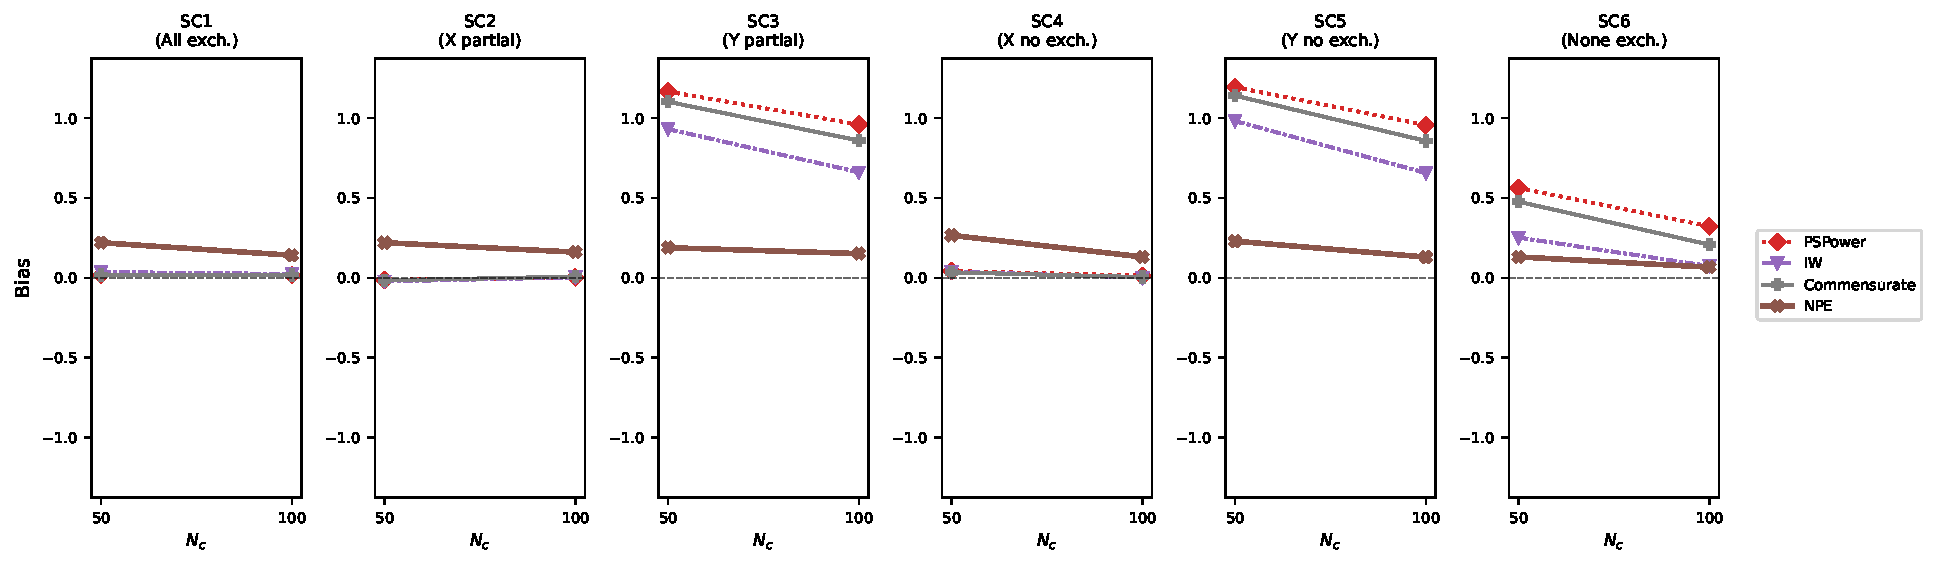
\includegraphics[width=.74\textwidth]{fig_bias.pdf}
    \caption{Bias across the six simulation scenarios for the non-null run.}
    \label{fig:sim-bias}
\end{figure}

\begin{figure}[!htbp]
    \centering
    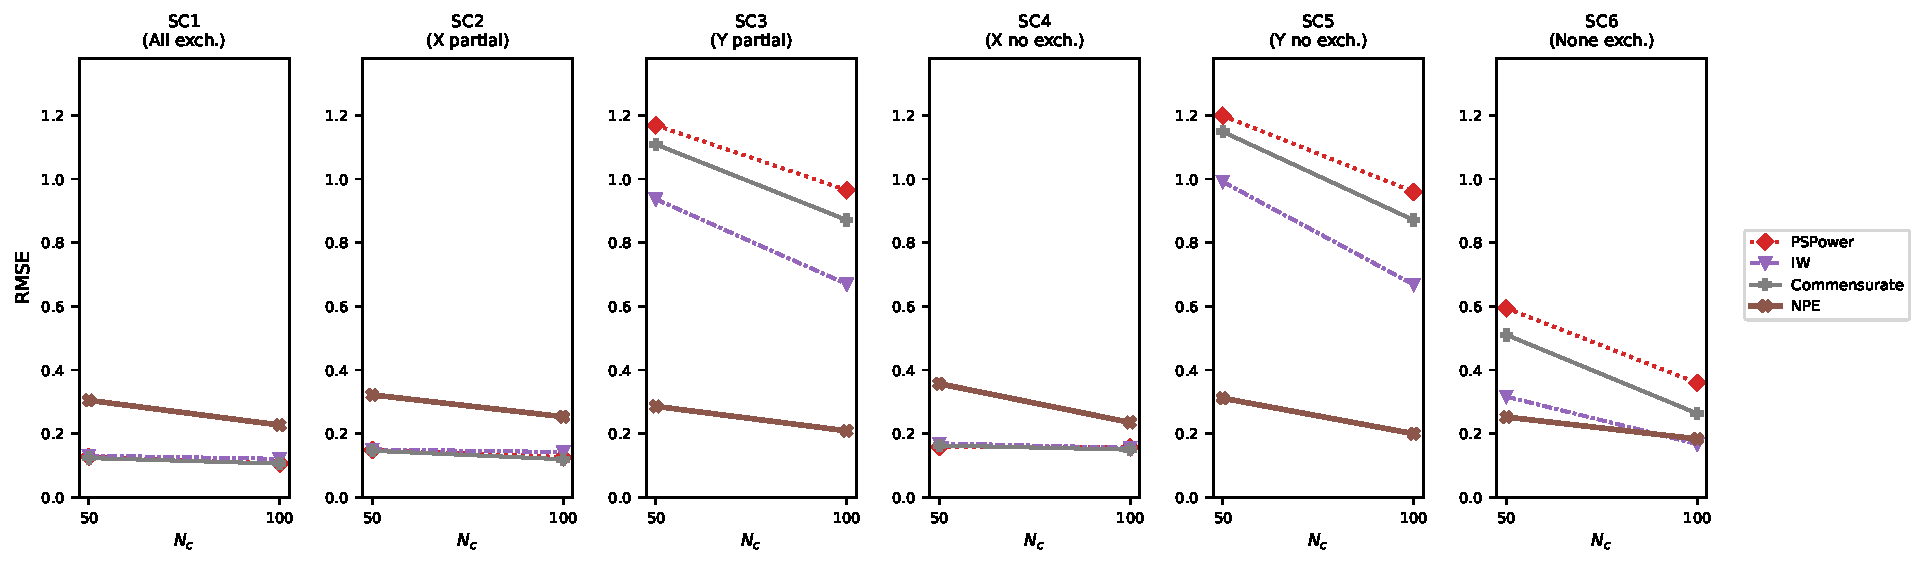
\includegraphics[width=.74\textwidth]{fig_rmse.pdf}
    \caption{RMSE across the six simulation scenarios for the non-null run.}
    \label{fig:sim-rmse}
\end{figure}

\begin{figure}[!htbp]
    \centering
    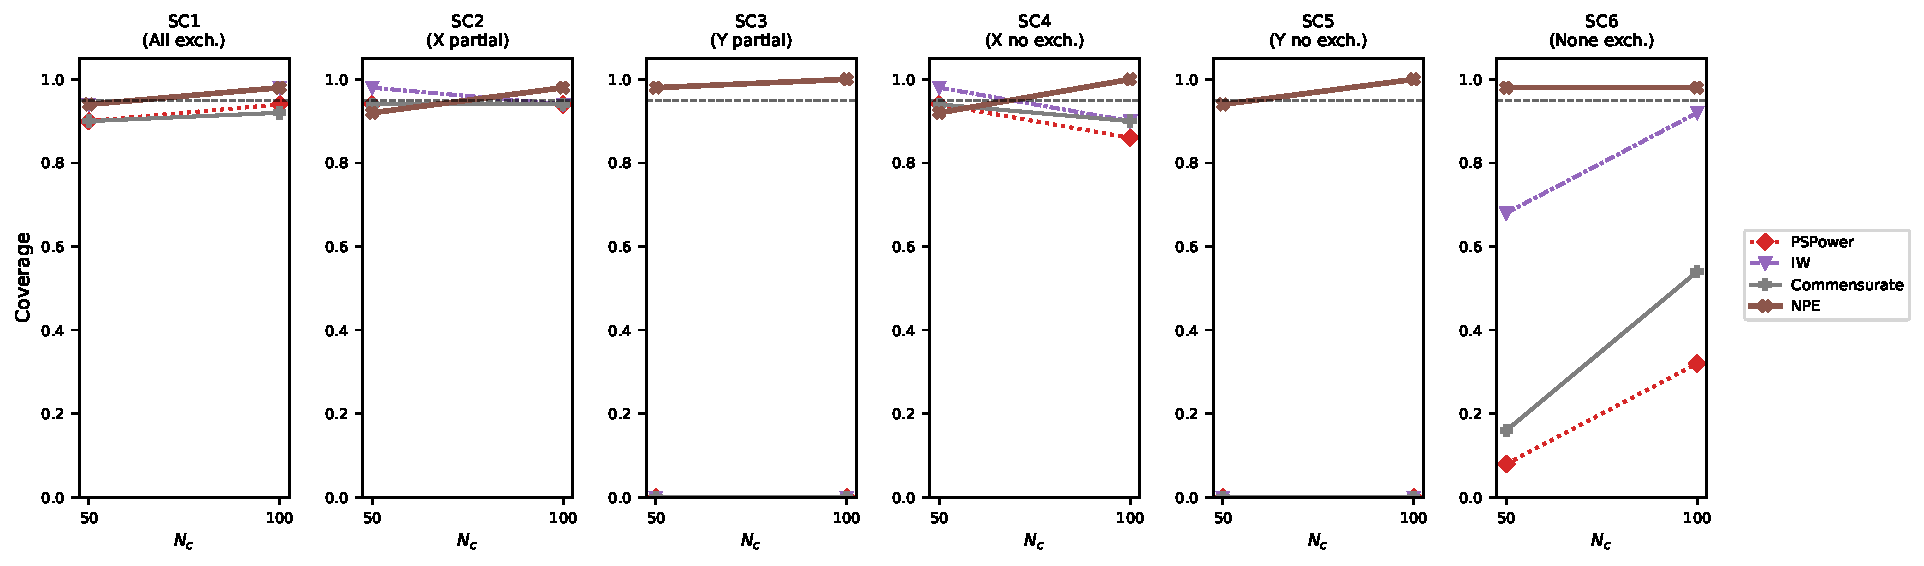
\includegraphics[width=.74\textwidth]{fig_coverage.pdf}
    \caption{Coverage across the six simulation scenarios for the non-null run.}
    \label{fig:sim-coverage}
\end{figure}

\begin{figure}[!htbp]
    \centering
    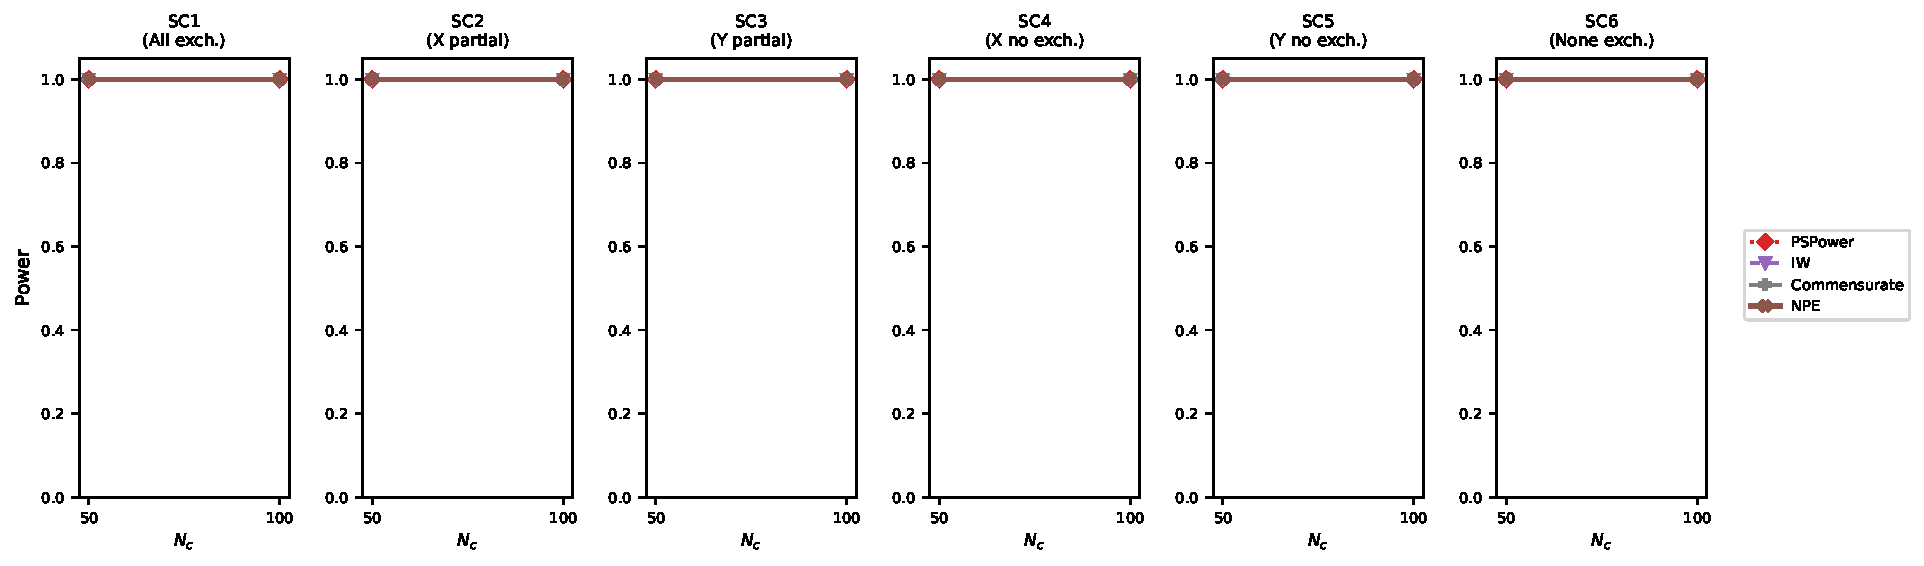
\includegraphics[width=.74\textwidth]{fig_power.pdf}
    \caption{Power across the six simulation scenarios for the non-null run.}
    \label{fig:sim-power}
\end{figure}

\subsection{Null results}

Table~\ref{tab:sim-null} summarizes the null run with $\theta=0$.
Here the main quantity of interest is Type I error.
In SC1 and SC2, the classical methods still have cleaner operating
characteristics, although NPE remains in a reasonable range.
The harder settings tell a different story.
In SC3, SC5, and SC6, the classical borrowing methods have very poor coverage
and severely inflated Type I error, while NPE stays much closer to nominal
behavior.

\begin{table*}[t]
\centering
\small
\caption{Null simulation results ($\theta = 0$).}
\label{tab:sim-null}
\begin{tabular}{llcccc}
\toprule
$N_c$ & Scenario & Method & Bias & RMSE & Coverage & Type I Error \\
\midrule
\multirow{24}{*}{50}
& SC1 & PSPower      & 0.0187 & 0.1269 & 0.90 & 0.10 \\
& SC1 & IW           & 0.0373 & 0.1311 & 0.94 & 0.06 \\
& SC1 & Commensurate & 0.0187 & 0.1235 & 0.90 & 0.10 \\
& SC1 & NPE          & 0.3172 & 0.3811 & 0.90 & 0.10 \\
\cmidrule(lr){2-7}
& SC2 & PSPower      & -0.0117 & 0.1485 & 0.94 & 0.06 \\
& SC2 & IW           & -0.0212 & 0.1503 & 0.98 & 0.02 \\
& SC2 & Commensurate & -0.0152 & 0.1463 & 0.94 & 0.06 \\
& SC2 & NPE          & 0.2954 & 0.3703 & 0.90 & 0.10 \\
\cmidrule(lr){2-7}
& SC3 & PSPower      & 1.1659 & 1.1698 & 0.00 & 1.00 \\
& SC3 & IW           & 0.9314 & 0.9377 & 0.00 & 1.00 \\
& SC3 & Commensurate & 1.1022 & 1.1096 & 0.00 & 1.00 \\
& SC3 & NPE          & 0.3333 & 0.4062 & 0.92 & 0.08 \\
\cmidrule(lr){2-7}
& SC4 & PSPower      & 0.0441 & 0.1582 & 0.96 & 0.04 \\
& SC4 & IW           & 0.0406 & 0.1700 & 0.98 & 0.02 \\
& SC4 & Commensurate & 0.0355 & 0.1632 & 0.94 & 0.06 \\
& SC4 & NPE          & 0.3495 & 0.4082 & 0.86 & 0.14 \\
\cmidrule(lr){2-7}
& SC5 & PSPower      & 1.1941 & 1.1997 & 0.00 & 1.00 \\
& SC5 & IW           & 0.9817 & 0.9923 & 0.00 & 1.00 \\
& SC5 & Commensurate & 1.1404 & 1.1493 & 0.00 & 1.00 \\
& SC5 & NPE          & 0.4052 & 0.4649 & 0.84 & 0.16 \\
\cmidrule(lr){2-7}
& SC6 & PSPower      & 0.5626 & 0.5952 & 0.08 & 0.92 \\
& SC6 & IW           & 0.2533 & 0.3176 & 0.68 & 0.32 \\
& SC6 & Commensurate & 0.4774 & 0.5114 & 0.18 & 0.82 \\
& SC6 & NPE          & 0.2874 & 0.3508 & 0.92 & 0.08 \\
\midrule
\multirow{24}{*}{100}
& SC1 & PSPower      & 0.0182 & 0.1063 & 0.94 & 0.06 \\
& SC1 & IW           & 0.0245 & 0.1206 & 0.98 & 0.02 \\
& SC1 & Commensurate & 0.0187 & 0.1059 & 0.92 & 0.08 \\
& SC1 & NPE          & 0.2542 & 0.3022 & 0.92 & 0.08 \\
\cmidrule(lr){2-7}
& SC2 & PSPower      & 0.0039 & 0.1262 & 0.94 & 0.06 \\
& SC2 & IW           & 0.0052 & 0.1422 & 0.94 & 0.06 \\
& SC2 & Commensurate & 0.0087 & 0.1195 & 0.94 & 0.06 \\
& SC2 & NPE          & 0.3132 & 0.3690 & 0.92 & 0.08 \\
\cmidrule(lr){2-7}
& SC3 & PSPower      & 0.9591 & 0.9655 & 0.00 & 1.00 \\
& SC3 & IW           & 0.6603 & 0.6707 & 0.00 & 1.00 \\
& SC3 & Commensurate & 0.8593 & 0.8721 & 0.00 & 1.00 \\
& SC3 & NPE          & 0.3574 & 0.3776 & 0.98 & 0.02 \\
\cmidrule(lr){2-7}
& SC4 & PSPower      & 0.0132 & 0.1576 & 0.86 & 0.14 \\
& SC4 & IW           & 0.0021 & 0.1551 & 0.92 & 0.08 \\
& SC4 & Commensurate & 0.0053 & 0.1497 & 0.90 & 0.10 \\
& SC4 & NPE          & 0.2651 & 0.3219 & 0.98 & 0.02 \\
\cmidrule(lr){2-7}
& SC5 & PSPower      & 0.9551 & 0.9601 & 0.00 & 1.00 \\
& SC5 & IW           & 0.6563 & 0.6687 & 0.00 & 1.00 \\
& SC5 & Commensurate & 0.8571 & 0.8716 & 0.00 & 1.00 \\
& SC5 & NPE          & 0.3322 & 0.3523 & 0.96 & 0.04 \\
\cmidrule(lr){2-7}
& SC6 & PSPower      & 0.3229 & 0.3601 & 0.32 & 0.68 \\
& SC6 & IW           & 0.0741 & 0.1675 & 0.92 & 0.08 \\
& SC6 & Commensurate & 0.2082 & 0.2638 & 0.54 & 0.46 \\
& SC6 & NPE          & 0.2651 & 0.3115 & 0.94 & 0.06 \\
\bottomrule
\end{tabular}
\end{table*}

\begin{figure}[!htbp]
    \centering
    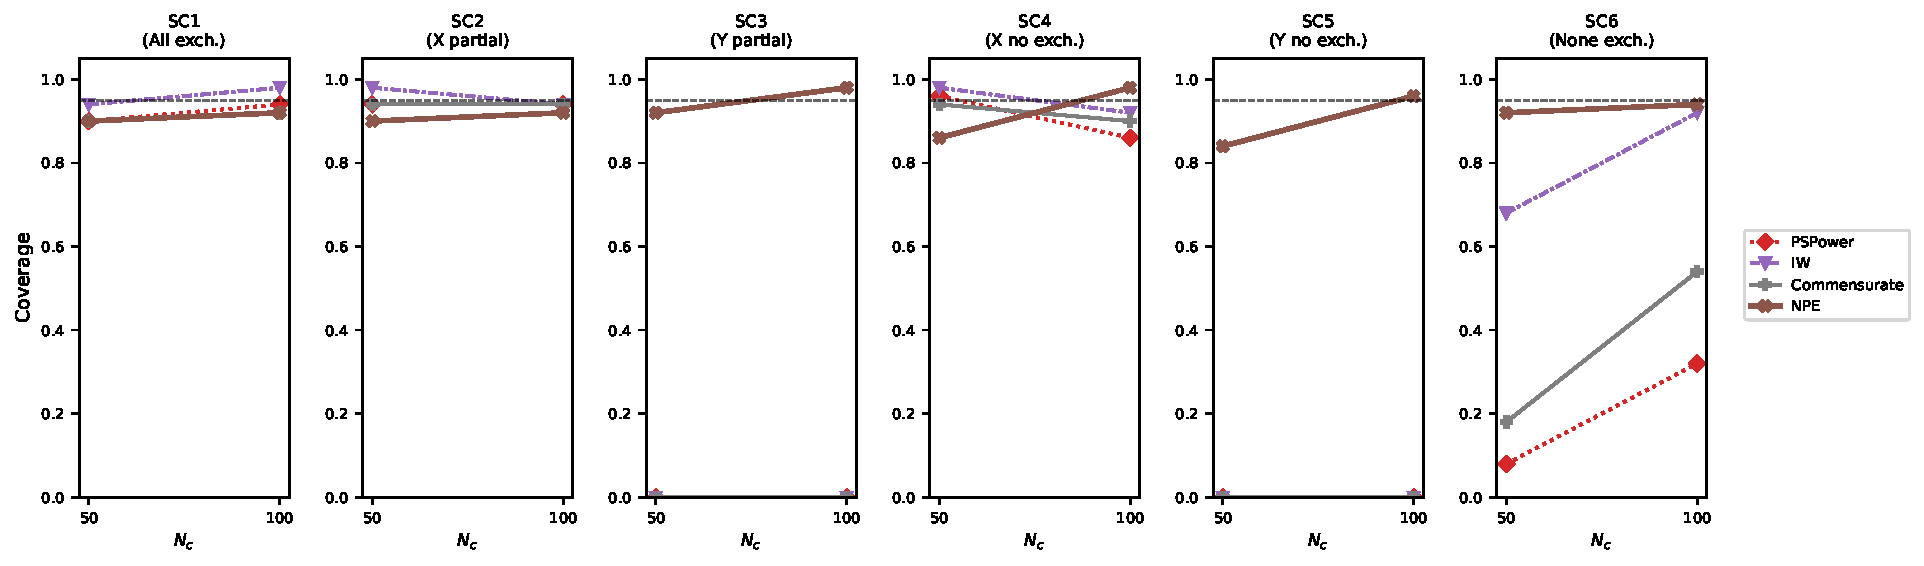
\includegraphics[width=.74\textwidth]{fig_coverage_null.pdf}
    \caption{Coverage across the six simulation scenarios for the null run.}
    \label{fig:sim-coverage-null}
\end{figure}

\begin{figure}[!htbp]
    \centering
    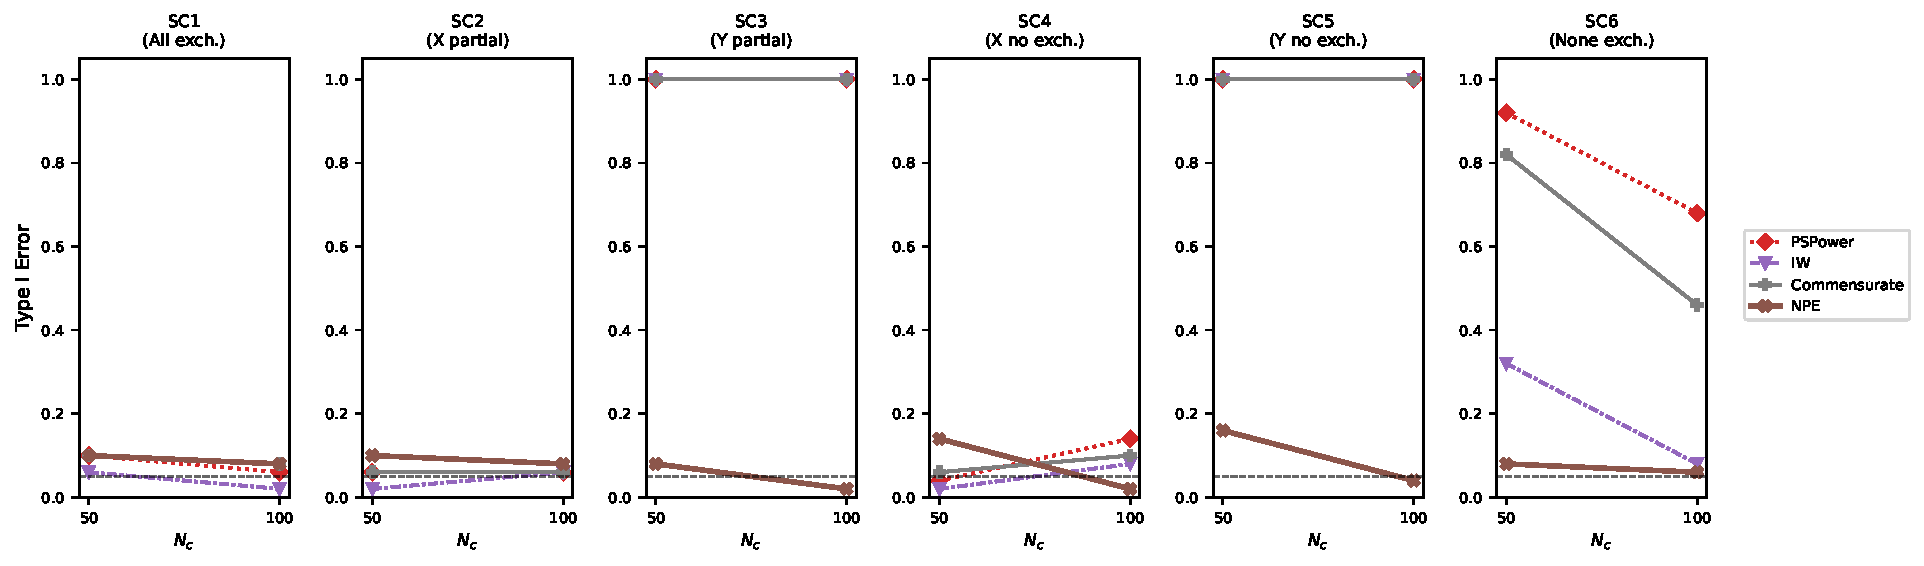
\includegraphics[width=.74\textwidth]{fig_type1_error.pdf}
    \caption{Type I error across the six simulation scenarios for the null run.}
    \label{fig:sim-type1}
\end{figure}

\subsection{Interpretation}

The simulation results do not suggest that NPE is best in every setting.
In SC1 and SC2, and in part of SC4, the classical methods are already stable
and often have smaller bias and RMSE.
The main advantage of NPE appears in the harder settings.
When the outcome model changes across sources, as in SC3 and SC5, or when both
covariate and outcome mismatch are present, as in SC6, the standard borrowing
methods can have large bias, poor coverage, and inflated Type I error.
NPE is much more stable there.

Taken together, these results suggest that NPE is most useful when source
mismatch is difficult to capture with a fixed borrowing rule, especially when the
main problem is outcome drift rather than mild covariate shift.
\section{Real-Data Example: ADNI}
\label{sec:adni}

We complement the simulation study with a real-data example based on the
Alzheimer's Disease Neuroimaging Initiative (ADNI). The purpose of this section
is different from that of the simulations. The simulations are used for
controlled methodological evaluation, whereas the ADNI analysis is meant to
show that the borrowing problem also appears clearly in an observed dataset.

ADNI is not a randomized treatment study, so we do not treat this section as a
treatment-effect analysis. Instead, we use it as a cohort-difference risk
problem. The question is whether borrowing from an earlier ADNI cohort would
pull inference away from the later concurrent cohort, and whether the proposed
NPE formulation can better recover the concurrent risk level.

\subsection{ADNI setup}

We define the external cohort as ADNI1 and the concurrent cohort as the pooled
ADNIGO and ADNI2 samples. The analysis is restricted to subjects with mild
cognitive impairment (MCI) at baseline. The outcome is conversion to dementia
(or Alzheimer's disease) by approximately 24 months. For subject $i$, let
\[
Y_i =
\begin{cases}
1, & \text{if subject } i \text{ converts by approximately 24 months},\\
0, & \text{otherwise.}
\end{cases}
\]

For each subject, we use the baseline covariate vector
\[
X_i = (\text{age},\ \text{female},\ \text{education},\ \text{APOE4 count},\
\text{MMSE}_{\mathrm{bl}},\ \text{ADAS13}_{\mathrm{bl}},\
\text{CDRSB}_{\mathrm{bl}},\ \text{FAQ}_{\mathrm{bl}}).
\]

Table~\ref{tab:adni-cohort-summary} summarizes the two cohorts. The concurrent
cohort contains 376 subjects with an event rate of 0.1702, whereas the
external cohort contains 337 subjects with an event rate of 0.3769. This
difference is large enough to make naive borrowing questionable.

\begin{table}[t]
\centering
\caption{ADNI cohort summary for the real-data borrowing example.}
\label{tab:adni-cohort-summary}
\begin{tabular}{lcc}
\toprule
Cohort & Number of subjects & Conversion rate \\
\midrule
Concurrent (ADNIGO + ADNI2) & 376 & 0.1702 \\
External (ADNI1)            & 337 & 0.3769 \\
\bottomrule
\end{tabular}
\end{table}

\subsection{Baseline benchmark}

Before applying NPE, we first check whether the data show the borrowing issue
we are trying to study. We fit repeated logistic-regression baselines and
evaluate them on a held-out concurrent test set:
\begin{itemize}
    \item \textbf{ConcurrentOnly}: trained only on concurrent data;
    \item \textbf{ExternalOnly}: trained only on external data;
    \item \textbf{Pooled}: trained on the combined external and concurrent data.
\end{itemize}

The results are shown in Table~\ref{tab:adni-baselines}. All three approaches
have similarly high AUC and accuracy, so the main issue is not ranking
performance. The more noticeable difference is calibration. The
\texttt{ExternalOnly} and \texttt{Pooled} models both predict risks that are
too high relative to the concurrent cohort. The observed concurrent event rate
is 0.168, while the corresponding mean predicted risks are 0.248 and 0.218.
This suggests that direct borrowing mainly distorts the level of risk rather
than discrimination.

\begin{table}[t]
\centering
\caption{Baseline benchmark on a held-out concurrent test set.}
\label{tab:adni-baselines}
\begin{tabular}{lcccccc}
\toprule
Method & AUC & Accuracy & Brier & LogLoss & MeanPred & MeanObs \\
\midrule
ConcurrentOnly & 0.918 & 0.881 & 0.084 & 0.271 & 0.183 & 0.168 \\
ExternalOnly   & 0.923 & 0.887 & 0.088 & 0.303 & 0.248 & 0.168 \\
Pooled         & 0.923 & 0.883 & 0.083 & 0.276 & 0.218 & 0.168 \\
\bottomrule
\end{tabular}
\end{table}

\subsection{ADNI-specific NPE formulation}

Since ADNI does not provide the same randomized treatment setting as the
simulation study, we use a simpler formulation in which the target is the
concurrent risk level. Let $X_c$ and $X_e$ denote the observed covariates in
the concurrent and external cohorts. We simulate outcomes according to
\begin{align}
Y_c &\sim \mathrm{Bernoulli}\!\left(\sigma(X_c\beta + \theta)\right), \\
Y_e &\sim \mathrm{Bernoulli}\!\left(\sigma(X_e\beta + \theta + \delta)\right),
\end{align}
where $\sigma(z)=1/(1+e^{-z})$ is the logistic link.

In this model, $\theta$ is the concurrent risk-level parameter of interest,
$\delta$ represents the shift between the external and concurrent outcome
levels, and $\beta$ denotes the covariate effects. The role of $\delta$ is
important here because it allows the external cohort to differ rather than
forcing full exchangeability.

To generate training data for NPE, we first fit a logistic model to the
observed ADNI data and use the fitted coefficient vector as an anchor
$\beta_{\mathrm{anchor}}$. We then simulate outcomes on the real ADNI
covariates by sampling
\[
\theta \sim \mathrm{Uniform}(-3,0), \qquad
\delta \sim N(0,0.75^2),
\]
adding small perturbations around $\beta_{\mathrm{anchor}}$, and generating
$Y_c$ and $Y_e$ on the fixed covariate matrices $X_c$ and $X_e$. For each
simulated dataset, we compute summary statistics based on covariate means and
standard deviations, event-rate summaries, between-cohort differences, and
sample-size information. The NPE model is then trained to approximate the
posterior distribution of $\theta$.

\subsection{ADNI results}

Table~\ref{tab:adni-main-results} shows the main ADNI result. The posterior
mean of the concurrent risk parameter is $-1.5990$, with posterior standard
deviation $0.8585$ and a 95\% interval of $(-3.3009,\ 0.1082)$. The observed
concurrent event rate is 0.1702, which corresponds to an empirical concurrent
logit risk of
\[
\mathrm{logit}(0.1702) \approx -1.5841.
\]
The NPE posterior mean is therefore very close to the empirical concurrent
target.

\begin{table}[t]
\centering
\caption{Main ADNI real-data result for the NPE-based formulation.}
\label{tab:adni-main-results}
\begin{tabular}{lc}
\toprule
Quantity & Value \\
\midrule
Posterior mean of $\theta$     & $-1.5990$ \\
Posterior SD of $\theta$       & $0.8585$ \\
95\% interval for $\theta$     & $(-3.3009,\ 0.1082)$ \\
Observed concurrent event rate & $0.1702$ \\
Observed external event rate   & $0.3769$ \\
Empirical concurrent logit     & $-1.5841$ \\
\bottomrule
\end{tabular}
\end{table}

Table~\ref{tab:adni-comparators} compares this estimate with several simple
reference values. The empirical external-only logit and pooled logit are both
substantially above the concurrent target. Even the offset-based MLE estimates
remain noticeably higher than the concurrent empirical logit. Among the
estimators considered here, the NPE posterior mean is the closest to the
concurrent target.

\begin{table}[t]
\centering
\caption{Comparator estimates in the ADNI real-data example.}
\label{tab:adni-comparators}
\begin{tabular}{lc}
\toprule
Estimator & Value \\
\midrule
Empirical logit (concurrent)        & $-1.5841$ \\
Empirical logit (external)          & $-0.5029$ \\
Empirical logit (pooled)            & $-1.0054$ \\
Offset-MLE $\theta$ (concurrent)    & $-1.0749$ \\
Offset-MLE $\theta$ (pooled)        & $-0.7240$ \\
Offset-MLE $\delta$ (external shift)& $0.6022$ \\
NPE posterior mean $\theta$         & $-1.5990$ \\
\bottomrule
\end{tabular}
\end{table}

Overall, the ADNI analysis supports the same broad message as the simulation
study. The earlier and later cohorts are not directly comparable, and direct
borrowing tends to push the estimated risk upward. The ADNI-specific NPE
formulation is much closer to the concurrent target. We do not view this as a
replacement for the simulation study, but rather as a concrete example showing
that the borrowing problem is not only a theoretical concern.
\section{Discussion}
\label{sec:discussion}

We studied neural posterior estimation as an amortized approach to Bayesian
dynamic borrowing: pretrain once on a broad simulation distribution, then obtain
posteriors for new current--external pairs in a single forward pass. The
simulation study isolates covariate shift, outcome drift, and their combination;
ADNI illustrates that cohort mismatch can pull inference away from the
concurrent target even when discrimination remains strong. The empirical scope
is a scalar current-study target---an additive study-effect parameter in the
Gaussian simulations and a cohort-level risk parameter in ADNI. Covariate
effects, treatment--covariate interactions, and other causal functionals require
additional evaluation; Appendix~\ref{app:covariate-effect} provides only a
limited illustrative check for one target-aware covariate-effect analysis. This
framing keeps the real-data example aligned with the estimand actually analyzed
rather than treating ADNI as a randomized treatment-effect study.

Posterior quality depends on the pretraining simulator, so mismatch patterns
outside its support cannot be handled reliably. The current hand-crafted
summaries expose auditable signals of covariate shift, outcome-mechanism drift,
overlap, and joint mismatch, but may miss richer patient-level structure.
Runnable code is included in the supplementary material; ADNI raw data require
separate data-use access. Future work will study richer paired-data
representations, such as patient-level encoders for irregular longitudinal
records, posterior-spread calibration in severe mismatch regimes, multi-source
borrowing, and broader evaluation across estimands and prospective
data-borrowing settings.

\newpage
\bibliography{refs}
\newpage
\appendix
\section{Additional Results}
\label{app:additional-results}

\subsection{Full Simulation Tables}

Tables~\ref{tab:sim-full-nonnull}--\ref{tab:sim-full-null-100} report the full
simulation results corresponding to the main-text figures.

\scriptsize
\setlength{\tabcolsep}{3pt}
\renewcommand{\arraystretch}{1.08}
\begin{longtable}{llccccc}
\caption{Full non-null simulation results ($\theta = 1$).}
\label{tab:sim-full-nonnull}\\
\toprule
$N_c$ & Scenario & Method & Bias & RMSE & Coverage & Power \\
\midrule
\endfirsthead
\toprule
$N_c$ & Scenario & Method & Bias & RMSE & Coverage & Power \\
\midrule
\endhead
50 & SC1 & PSPower      & 0.0183 & 0.1268 & 0.90 & 1.00 \\
& SC1 & IW           & 0.0365 & 0.1309 & 0.94 & 1.00 \\
& SC1 & Commensurate & 0.0183 & 0.1234 & 0.90 & 1.00 \\
& SC1 & NPE          & 0.2201 & 0.3049 & 0.94 & 1.00 \\
\cmidrule(lr){2-7}
& SC2 & PSPower      & -0.0126 & 0.1485 & 0.94 & 1.00 \\
& SC2 & IW           & -0.0223 & 0.1505 & 0.98 & 1.00 \\
& SC2 & Commensurate & -0.0160 & 0.1464 & 0.94 & 1.00 \\
& SC2 & NPE          & 0.2202 & 0.3219 & 0.92 & 1.00 \\
\cmidrule(lr){2-7}
& SC3 & PSPower      & 1.1655 & 1.1693 & 0.00 & 1.00 \\
& SC3 & IW           & 0.9306 & 0.9369 & 0.00 & 1.00 \\
& SC3 & Commensurate & 1.1016 & 1.1091 & 0.00 & 1.00 \\
& SC3 & NPE          & 0.1889 & 0.2859 & 0.98 & 1.00 \\
\cmidrule(lr){2-7}
& SC4 & PSPower      & 0.0432 & 0.1579 & 0.94 & 1.00 \\
& SC4 & IW           & 0.0394 & 0.1697 & 0.98 & 1.00 \\
& SC4 & Commensurate & 0.0347 & 0.1630 & 0.94 & 1.00 \\
& SC4 & NPE          & 0.2661 & 0.3570 & 0.92 & 1.00 \\
\cmidrule(lr){2-7}
& SC5 & PSPower      & 1.1936 & 1.1993 & 0.00 & 1.00 \\
& SC5 & IW           & 0.9810 & 0.9915 & 0.00 & 1.00 \\
& SC5 & Commensurate & 1.1399 & 1.1488 & 0.00 & 1.00 \\
& SC5 & NPE          & 0.2298 & 0.3115 & 0.94 & 1.00 \\
\cmidrule(lr){2-7}
& SC6 & PSPower      & 0.5617 & 0.5943 & 0.08 & 1.00 \\
& SC6 & IW           & 0.2521 & 0.3167 & 0.68 & 1.00 \\
& SC6 & Commensurate & 0.4765 & 0.5107 & 0.16 & 1.00 \\
& SC6 & NPE          & 0.1311 & 0.2523 & 0.98 & 1.00 \\
\midrule
100 & SC1 & PSPower      & 0.0178 & 0.1063 & 0.94 & 1.00 \\
& SC1 & IW           & 0.0238 & 0.1205 & 0.98 & 1.00 \\
& SC1 & Commensurate & 0.0183 & 0.1058 & 0.92 & 1.00 \\
& SC1 & NPE          & 0.1413 & 0.2270 & 0.98 & 1.00 \\
\cmidrule(lr){2-7}
& SC2 & PSPower      & 0.0032 & 0.1261 & 0.94 & 1.00 \\
& SC2 & IW           & 0.0044 & 0.1422 & 0.94 & 1.00 \\
& SC2 & Commensurate & 0.0081 & 0.1195 & 0.94 & 1.00 \\
& SC2 & NPE          & 0.1610 & 0.2532 & 0.98 & 1.00 \\
\cmidrule(lr){2-7}
& SC3 & PSPower      & 0.9587 & 0.9651 & 0.00 & 1.00 \\
& SC3 & IW           & 0.6597 & 0.6701 & 0.00 & 1.00 \\
& SC3 & Commensurate & 0.8586 & 0.8714 & 0.00 & 1.00 \\
& SC3 & NPE          & 0.1518 & 0.2089 & 1.00 & 1.00 \\
\cmidrule(lr){2-7}
& SC4 & PSPower      & 0.0125 & 0.1576 & 0.86 & 1.00 \\
& SC4 & IW           & 0.0013 & 0.1552 & 0.90 & 1.00 \\
& SC4 & Commensurate & 0.0047 & 0.1497 & 0.90 & 1.00 \\
& SC4 & NPE          & 0.1312 & 0.2352 & 1.00 & 1.00 \\
\cmidrule(lr){2-7}
& SC5 & PSPower      & 0.9547 & 0.9597 & 0.00 & 1.00 \\
& SC5 & IW           & 0.6557 & 0.6681 & 0.00 & 1.00 \\
& SC5 & Commensurate & 0.8564 & 0.8710 & 0.00 & 1.00 \\
& SC5 & NPE          & 0.1299 & 0.1998 & 1.00 & 1.00 \\
\cmidrule(lr){2-7}
& SC6 & PSPower      & 0.3222 & 0.3595 & 0.32 & 1.00 \\
& SC6 & IW           & 0.0733 & 0.1672 & 0.92 & 1.00 \\
& SC6 & Commensurate & 0.2075 & 0.2633 & 0.54 & 1.00 \\
& SC6 & NPE          & 0.0668 & 0.1835 & 0.98 & 1.00 \\
\bottomrule
\end{longtable}
\normalsize

\begin{table*}[p]
\centering
\scriptsize
\setlength{\tabcolsep}{5pt}
\renewcommand{\arraystretch}{1.08}
\caption{Full null simulation results ($\theta = 0$) for $N_c=50$.}
\label{tab:sim-full-null-50}
\begin{tabular}{llcccc}
\toprule
Scenario & Method & Bias & RMSE & Coverage & Type I Error \\
\midrule
SC1 & PSPower      & 0.0187 & 0.1269 & 0.90 & 0.10 \\
SC1 & IW           & 0.0373 & 0.1311 & 0.94 & 0.06 \\
SC1 & Commensurate & 0.0187 & 0.1235 & 0.90 & 0.10 \\
SC1 & NPE          & 0.3172 & 0.3811 & 0.90 & 0.10 \\
\cmidrule(lr){1-6}
SC2 & PSPower      & -0.0117 & 0.1485 & 0.94 & 0.06 \\
SC2 & IW           & -0.0212 & 0.1503 & 0.98 & 0.02 \\
SC2 & Commensurate & -0.0152 & 0.1463 & 0.94 & 0.06 \\
SC2 & NPE          & 0.2954 & 0.3703 & 0.90 & 0.10 \\
\cmidrule(lr){1-6}
SC3 & PSPower      & 1.1659 & 1.1698 & 0.00 & 1.00 \\
SC3 & IW           & 0.9314 & 0.9377 & 0.00 & 1.00 \\
SC3 & Commensurate & 1.1022 & 1.1096 & 0.00 & 1.00 \\
SC3 & NPE          & 0.3333 & 0.4062 & 0.92 & 0.08 \\
\cmidrule(lr){1-6}
SC4 & PSPower      & 0.0441 & 0.1582 & 0.96 & 0.04 \\
SC4 & IW           & 0.0406 & 0.1700 & 0.98 & 0.02 \\
SC4 & Commensurate & 0.0355 & 0.1632 & 0.94 & 0.06 \\
SC4 & NPE          & 0.3495 & 0.4082 & 0.86 & 0.14 \\
\cmidrule(lr){1-6}
SC5 & PSPower      & 1.1941 & 1.1997 & 0.00 & 1.00 \\
SC5 & IW           & 0.9817 & 0.9923 & 0.00 & 1.00 \\
SC5 & Commensurate & 1.1404 & 1.1493 & 0.00 & 1.00 \\
SC5 & NPE          & 0.4052 & 0.4649 & 0.84 & 0.16 \\
\cmidrule(lr){1-6}
SC6 & PSPower      & 0.5626 & 0.5952 & 0.08 & 0.92 \\
SC6 & IW           & 0.2533 & 0.3176 & 0.68 & 0.32 \\
SC6 & Commensurate & 0.4774 & 0.5114 & 0.18 & 0.82 \\
SC6 & NPE          & 0.2874 & 0.3508 & 0.92 & 0.08 \\
\bottomrule
\end{tabular}
\end{table*}

\begin{table*}[p]
\centering
\scriptsize
\setlength{\tabcolsep}{5pt}
\renewcommand{\arraystretch}{1.08}
\caption{Full null simulation results ($\theta = 0$) for $N_c=100$.}
\label{tab:sim-full-null-100}
\begin{tabular}{llcccc}
\toprule
Scenario & Method & Bias & RMSE & Coverage & Type I Error \\
\midrule
SC1 & PSPower      & 0.0182 & 0.1063 & 0.94 & 0.06 \\
SC1 & IW           & 0.0245 & 0.1206 & 0.98 & 0.02 \\
SC1 & Commensurate & 0.0187 & 0.1059 & 0.92 & 0.08 \\
SC1 & NPE          & 0.2542 & 0.3022 & 0.92 & 0.08 \\
\cmidrule(lr){1-6}
SC2 & PSPower      & 0.0039 & 0.1262 & 0.94 & 0.06 \\
SC2 & IW           & 0.0052 & 0.1422 & 0.94 & 0.06 \\
SC2 & Commensurate & 0.0087 & 0.1195 & 0.94 & 0.06 \\
SC2 & NPE          & 0.3132 & 0.3690 & 0.92 & 0.08 \\
\cmidrule(lr){1-6}
SC3 & PSPower      & 0.9591 & 0.9655 & 0.00 & 1.00 \\
SC3 & IW           & 0.6603 & 0.6707 & 0.00 & 1.00 \\
SC3 & Commensurate & 0.8593 & 0.8721 & 0.00 & 1.00 \\
SC3 & NPE          & 0.3574 & 0.3776 & 0.98 & 0.02 \\
\cmidrule(lr){1-6}
SC4 & PSPower      & 0.0132 & 0.1576 & 0.86 & 0.14 \\
SC4 & IW           & 0.0021 & 0.1551 & 0.92 & 0.08 \\
SC4 & Commensurate & 0.0053 & 0.1497 & 0.90 & 0.10 \\
SC4 & NPE          & 0.2651 & 0.3219 & 0.98 & 0.02 \\
\cmidrule(lr){1-6}
SC5 & PSPower      & 0.9551 & 0.9601 & 0.00 & 1.00 \\
SC5 & IW           & 0.6563 & 0.6687 & 0.00 & 1.00 \\
SC5 & Commensurate & 0.8571 & 0.8716 & 0.00 & 1.00 \\
SC5 & NPE          & 0.3322 & 0.3523 & 0.96 & 0.04 \\
\cmidrule(lr){1-6}
SC6 & PSPower      & 0.3229 & 0.3601 & 0.32 & 0.68 \\
SC6 & IW           & 0.0741 & 0.1675 & 0.92 & 0.08 \\
SC6 & Commensurate & 0.2082 & 0.2638 & 0.54 & 0.46 \\
SC6 & NPE          & 0.2651 & 0.3115 & 0.94 & 0.06 \\
\bottomrule
\end{tabular}
\end{table*}
\normalsize
\renewcommand{\arraystretch}{1}



\end{document}
